%%
%% Author: thompson
%% 26.10.17
%%

% Preamble
\documentclass[11pt]{article}

% Packages
\usepackage{a4wide}
\usepackage[utf8]{inputenc}
\usepackage[ngerman]{babel}
\usepackage{scrextend}      % Intending
\usepackage{graphicx}

% Document
\begin{document}

\section{ISO-OSI Referenzmodel}
    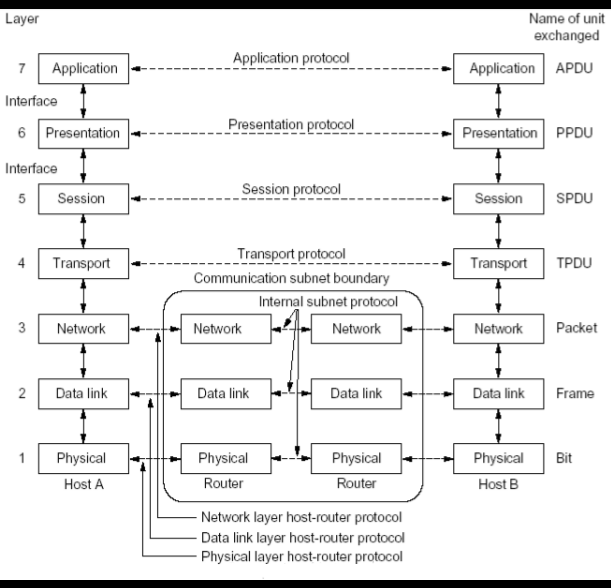
\includegraphics[width=\textwidth]{ISO_OSIReferenceModel.png}

    Das ISO-OSI Referenzmodell besteht aus verschiedenen Anwendungsschichten:
    \begin{enumerate}
        \item Physical Layer\\
        Dieser Layer beschreibt die fundamentale Netzwerkkommunikation. Datentransfer via
        physischem Layer sind reine Bitstreams.

        Hardware:
        \begin{addmargin}[1em]{1em}
            PHY-Chip: Ein PHY implementiert die Funktionen Senden und Empfangen von Daten zwischen
            Geräten mithilfe des Datalink Layers (MAC, LLC). Es enkodiert und dekodiert einkommende
            Übertragungen und Galvanische Trennung (Blockt ungewollten Datenempfang).
        \end{addmargin}

        Protokolle:
        \begin{addmargin}[1em]{1em}
            Integrated Services Digital Network: Internationaler Standard für Datenübertragung \& Telefonie
            Universal Serial Bus: Bussystem von Verbindungen um Daten zu übertragen
            Bluetooth, Ethernet, ...
        \end{addmargin}

        Normen: % TODO, found fucking nothing

        \item Data Link Layer\\
        Der Datenlink nutzt Frames zur Übertragung von Datensätzen. Frames bestehen aus einer gewissen Anzahl
        an Bit-Blöcken und einer Prüfsumme, welche die korrekte Datenflussübertragung gewährleistet.
        Fehlerbehafte Frames können anhand dieser Summe erkannt werden und der DLL kann das jeweilige Paket verwerfen
        oder sogar korrigieren.
        Im Falle des Verwerfens ist es allerdings nicht vorgesehen das jeweilige Frame neu anzufordern.

        Mithilfe der 'Data Flow Control' kann man die Dynamik der Frameübertragung steuern, etwa wie schnell
        Blöcke verschickt werden.

        Hardware:
        \begin{addmargin}[1em]{1em} % Left & right
            Bridge \& Switch: Arbeiten via Media Access Control(Mac) oder Logical Link Control(LLC).\\
            Die MAC-Bridge schützt gegen Kollisionen via Aufteilung des Netzes in verschiedene Kollisionsdomänen, d.H.
            ein Paket geht nur in das Netz, in welchem sich der tatsächliche Empfänger befindet.\\
            Die LLC-Bridge dient der Koppelung zweier Teilnetze mithilfe verschiedener Zugriffsverfahren, wie
            Token-Passing (Tokens werden zwischen Sendern gewechselt und dementsprechend startet Datenverkehr) oder
            Carrier Sense Multiple Access/Collision Detection (CSMA/CD; Typischer Router mit x-Medien).\\
        \end{addmargin}

        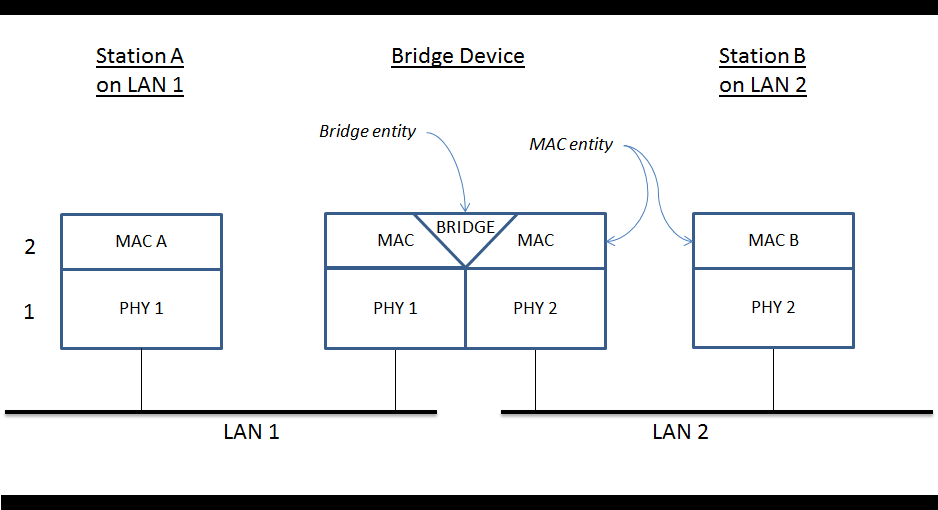
\includegraphics[width=\textwidth]{Network_Bridging.png}
        \footnote[1\small \emph{Schemata of Bridge/Switch inside a Network}]{By Crvincenzi - MS Powerpoint, CC BY-SA 3.0, https://commons.wikimedia.org/w/index.php?curid=25610536}

        Protokolle:
        \begin{addmargin}[1em]{1em}
            HDLC - High-Level Data Link Control: Transmition of sync/async frames\\
            SDLC - Synchronous Data Link Control: Bitsynchron \& Serielle Übertragung\\
            DDCMP - Digital Data Communications Message Protocol: Point-to-Point Transfer (Sicherheit)\\
            SPB - Shortest Path Bridging: Aufbau \& Konfig. + Multipath Routing\\
        \end{addmargin}

        Normen: IEEE, FDDI, ISO\\

        \item Network Layer
        Der Network Layer behandelt Weiterleitung und Routing durch multiple Zwischenmedien innerhalb
        eines Netzwerkes.

        Funktionen:
        \begin{addmargin}[1em]{1em}
            - CL-mode: Verbindungslose Kommunikation, über IP\\
            - Hostadressierung, jeder Host ist einzigartig identifizierbar\\
            - Weiterleitung: Partitionierung von Netzwerken in Subnetzwerke und Weiterleitung
            von Daten über Gateways und Router\\
        \end{addmargin}

        \item Transport Layer
        Die Transportschicht beschreibt den konkreten Datentransfer von A nach B.

        Protokolle:
        \begin{addmargin}[1em]{1em}
            - Transmission Control Protocol: TCP/IP - Datentransfer wird kontrolliert weitergegeben. Wird das Paket falsch oder garnicht
            empfangen, so wird eine Anfrage geschickt welche das Datenpaket neu schickt.
            Es gibt Flow- und Congestioncontrol. Grundsätzlich genutzt bei HTTP, FTP, SMTP.\\
            - User Datagram Protocol: UDP/IP - Datentransfer wird losgeschickt, ohne Kontrolle ob das Datenpaket tatsächlich ankommt.
            Es gibt also weder Flow- noch Congestioncontrol.\\
        \end{addmargin}

        \item Session Layer

        \item Presentation Layer

        \item Application Layer

    \end{enumerate}

    Die 5. und 6. Schicht wird meist impliziert, bzw. wird von der Praxis nicht angenommen.

\end{document}